\documentclass[12pt]{article}
\usepackage{listings}
\usepackage[frenchb]{babel}
\usepackage[utf8]{inputenc}
\usepackage[T1]{fontenc}
\usepackage{lmodern}
\usepackage{graphicx}
\usepackage{tikz}
\usepackage{algorithmic}
\usepackage{xcolor}
\usepackage{color}
\usepackage{amsmath}
\usepackage{amsfonts}
\usepackage{amssymb}
\usepackage{url}
\usepackage[linesnumbered, ruled, french, onelanguage]{algorithm2e}
\makeatletter
\g@addto@macro{\@algocf@init}{\SetKwInput{KwOut}{Sortie}}
\makeatother
\usepackage{geometry}
\usepackage{hyperref}
\definecolor{codegreen}{rgb}{0,0.6,0}
\definecolor{codegray}{rgb}{0.5,0.5,0.5}
\definecolor{codepurple}{rgb}{0.58,0,0.82}
\definecolor{backcolour}{rgb}{0.95,0.95,0.92}

\lstdefinestyle{mystyle}{
backgroundcolor=\color{backcolour},
commentstyle=\color{codegreen},
keywordstyle=\color{magenta},
numberstyle=\tiny\color{codegray},
stringstyle=\color{codepurple},
basicstyle=\ttfamily\footnotesize,
breakatwhitespace=false,
breaklines=true,
captionpos=b,
keepspaces=true,
numbers=left,
numbersep=5pt,
showspaces=false,
showstringspaces=false,
showtabs=false,
tabsize=2
}

\lstset{style=mystyle}

\hypersetup{pdftoolbar=true, colorlinks=true, linkcolor=black, 
    citecolor=black, filecolor=black, urlcolor=black
}

\begin{document}
\begin{titlepage}
\begin{center}
\vspace*{0cm}
\Huge\bf{Rapport de Projet} \\
\vspace*{1cm}
\LARGE{Méthode de conception : Jeu de Stratégie}\\
\vspace*{0.5cm}


\end{center}
\vspace*{0.7cm}
\begin{center}
\Large{Georges Dosseh 22012628\\
Idres Anis 22212192\\
Aidi Mohammed 22309377\\
Rezala Ayoub 22309776\\}
\vspace*{2cm}

\end{center}
\vspace*{1cm}

\begin{center}
\begin{minipage}[t]{0.48\textwidth}
\centering
\vspace*{0cm}

\includegraphics[width=3cm,height=3cm]{images/unicaen.png}

\vspace*{0.25cm}
\large{Université de Caen Normandie}
\large{UFR des Sciences}
\large{Département Informatique}\\
\large{3ème année de licence d’informatique}


\end{minipage}
\hfill
\end{center}
\end{titlepage}


%------------------------------
%sommaire
%------------------------------

\newpage

\tableofcontents

\newpage

%------------------------------
%contenu
%------------------------------

\section{Présentation du projet}

Le projet consiste à développer un jeu de stratégie au tour par tour. Chaque joueur évolue sur une grille et utilise diverses armes pour éliminer ses adversaires, avec pour objectif de rester le dernier survivant.\\
Les joueurs sont éliminés lorsqu’ils n’ont plus de points de vie. Durant leur tour, ils disposent d’un nombre limité d’actions qu’ils peuvent utiliser pour se déplacer, attaquer, activer un bouclier ou réaliser d’autres actions.\\
Un joueur peut effectuer autant d'actions qu’il le souhaite tant qu’il lui reste des points d’action. Son tour se termine lorsqu’il n’a plus de points d’action ou choisit volontairement de passer sans utiliser le reste de ses actions.

\section{Structure MVC (Modèle/Vue/Contrôleur)}

L'application est organisée selon l'architecture MVC, répartie en quatre packages principaux :  
\begin{itemize}
    \item \textbf{Modèle} : Contient les classes gérant la logique du jeu et les données essentielles, telles que les joueurs, les règles et les éléments de la grille.  
    \item \textbf{Vue} : Regroupe les composants d'affichage et l’interface utilisateur, permettant aux joueurs d’interagir avec le jeu via des éléments graphiques.  
    \item \textbf{Contrôleur} : Assure la communication entre le modèle et la vue, en capturant les actions des joueurs et en mettant à jour l'affichage en fonction des changements dans le jeu.  
    \item \textbf{Patterns} : Regroupe les classes mettant en œuvre divers design patterns (comme le \textit{Proxy}, \textit{Strategy} ou \textit{Factory}), facilitant la modularité, la réutilisabilité et la gestion des comportements spécifiques dans le jeu.  
\end{itemize}

Cette organisation garantit une séparation claire des responsabilités, rendant le code plus maintenable et évolutif.

\section{Compréhension de la conception logicielle}
\subsection{Modèle et patterns}
Cette section présente les différents modèles et patterns utilisés dans l'application pour structurer le code, faciliter son évolution, et optimiser les fonctionnalités.
\subsubsection{Modèle}

Le modèle représente la logique centrale et les données essentielles de l'application. Voici les principaux éléments qui structurent le modèle :

\begin{itemize}
    \item \textbf{Gestion de la grille (\texttt{PrincipalGrid} et \texttt{Grid})} :  
    Ces classes encapsulent la logique de la grille principale du jeu, comprenant la gestion des cases (libres ou occupées), des obstacles (\texttt{Mur}), et des éléments interactifs comme les bonus (\texttt{Pastille}), mines, ou bombes.  
    La classe \texttt{RandomGridGeneretor} permet de générer une grille procédurale selon des paramètres définis.

    \item \textbf{Représentation des joueurs (\texttt{Player})} :  
    Gère les attributs d'un joueur tels que ses points de vie, ses munitions et sa position.  
    Les joueurs peuvent interagir avec la grille et utiliser des armes (\texttt{Weapon}), comme des fusils (\texttt{Fuisil}), des bombes (\texttt{Bomb}) ou des mines.

    \item \textbf{Paramétrage global (\texttt{GameConfig})} :  
    Cette classe centralise les constantes du jeu, comme les dommages des armes ou les dimensions de la grille. Les paramètres sont configurables via un fichier externe, rendant l'application adaptable sans recompilation.

    \item \textbf{Interactions dynamiques} :  
    La classe \texttt{PrintThread} gère les actions liées à l'affichage ou au suivi en temps réel. Les mouvements des joueurs sont régis par des directions (\texttt{Direction}), et les interactions avec les éléments de la grille suivent des règles prédéfinies.
\end{itemize}

Ce modèle est conçu pour être extensible et maintenable, avec une gestion claire des responsabilités entre les différentes entités du jeu.

\subsubsection{Paramétrage du jeu}
Le jeu utilise plusieurs constantes que nous souhaitons pouvoir modifier facilement à travers toute l’application.
Pour cela, un fichier de configuration texte est utilisé. Chaque ligne du fichier suit un format tel que \textit{"BOMB-DAMAGE=5"}. La classe \texttt{GameConfig} lit ce fichier et stocke les valeurs dans des variables statiques, accessibles depuis n’importe quelle classe.
Ainsi, pour modifier une constante, il suffit de mettre à jour le fichier de configuration et de relancer l’application, sans nécessiter de recompilation. De plus, cette approche permet à l'utilisateur d’ajuster les paramètres selon ses préférences, sans toucher au code source.

\subsubsection{Pattern Factory}
L’instanciation des différents types de joueurs est gérée par la classe \texttt{PlayerFactory}, qui dispose d’une méthode \texttt{build()} retournant une instance de \texttt{Player} configurée avec divers paramètres.
Cela permet de créer facilement des archétypes de joueurs en définissant des méthodes spécifiques qui appellent \texttt{build()} avec des paramètres prédéfinis, par exemple pour générer un joueur doté d’un bonus de points de vie mais disposant de moins de munitions.
Actuellement, les archétypes sont identifiés par une chaîne de caractères dans un attribut de \texttt{Player}. Une amélioration envisageable serait de rendre la classe \texttt{Player} abstraite et d’utiliser la factory pour instancier des sous-classes représentant ces archétypes.

\begin{figure}[!h] \centering 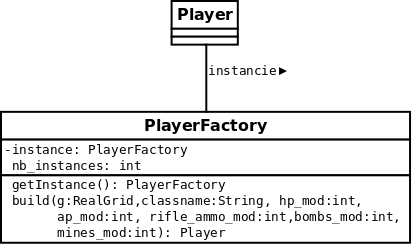
\includegraphics[scale=0.5]{images/factory.png} \caption{Pattern Factory pour les joueurs} \end{figure}

\subsubsection{Pattern Proxy}
Pour optimiser la gestion des données, une seule grille centralisée (\texttt{RealGrid}) stocke l’ensemble des informations du jeu. Toutefois, chaque joueur doit avoir une vue partielle de la grille, limitée aux éléments qu’il a lui-même découverts ou placés (comme les explosifs).
Le pattern Proxy permet de répondre à ces besoins en créant une classe \texttt{PlayerGrid} associée à chaque joueur. Cette classe est liée à la \texttt{RealGrid} unique, mais elle adapte les informations visibles en fonction des permissions du joueur.
Par exemple, la méthode \texttt{getTileAt()} de \texttt{PlayerGrid} intercepte l’appel pour vérifier si le joueur a le droit de voir la case demandée. Si ce n’est pas le cas, une case vide est retournée. De la même manière, \texttt{toString()} génère une représentation adaptée à la vision du joueur.

\begin{figure}[!h] \centering 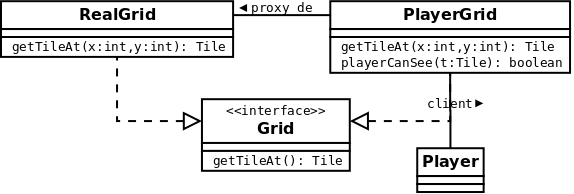
\includegraphics[scale=0.3]{images/proxy.png} \caption{Pattern Proxy pour les vues joueur} \end{figure}

\subsubsection{Pattern Strategy}

Le pattern \textit{Strategy} est utilisé à plusieurs endroits dans l'application pour offrir une flexibilité dans les comportements et les algorithmes. Voici les principales utilisations :

\paragraph{Génération de la grille :}
L'interface \texttt{GridStrategy} définit une méthode abstraite \texttt{generate()}, permettant de créer différents algorithmes de génération de grilles. Par exemple, la classe \texttt{RandomStrategy} implémente cette interface pour générer une grille avec des obstacles et éléments placés aléatoirement. Cette approche facilite l'ajout de nouvelles stratégies (comme une grille symétrique ou basée sur des motifs prédéfinis) sans modifier le code existant.

\paragraph{Comportement des joueurs :}
Une autre utilisation du pattern \textit{Strategy} est représentée par l'interface \texttt{PlayerStrategy}. Elle permet de définir différents comportements pour les joueurs. Par exemple, un joueur humain peut être contrôlé directement, tandis qu'un joueur robot suit une stratégie automatique pour ses déplacements et ses actions.

\begin{figure}[!h] \centering 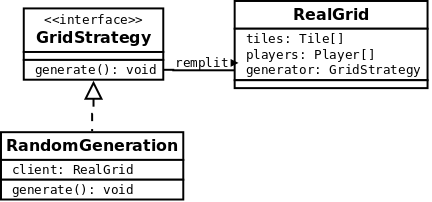
\includegraphics[scale=0.5]{images/strategy.png} \caption{Pattern Strategy pour la génération de grille} \end{figure}

\subsection{Contrôleur}

Le contrôleur de l'application, représenté par la classe \texttt{GameController}, gère la logique de jeu, l'ajout de joueurs et le chargement de la grille de jeu. Il agit comme une interface entre le modèle de données et les vues, assurant la mise à jour de l'état du jeu et la gestion des interactions.

La classe \texttt{GameController} est responsable de plusieurs tâches essentielles :

\begin{itemize}
    \item **Gestion de la grille** : Le contrôleur maintient une référence à la grille de jeu via l'objet \texttt{PrincipalGrid}, permettant de manipuler et de récupérer l'état de la grille.
    \item **Ajout de joueurs** : Le contrôleur ajoute des joueurs à la partie et associe une image représentative à chaque joueur grâce à la méthode \texttt{addPlayer()}. Les joueurs sont stockés dans un \texttt{HashMap} associant chaque joueur à son image.
    \item **Chargement de la grille** : Le contrôleur est également responsable du chargement de la grille à partir d'un fichier XML via la méthode \texttt{loadGrid()}. Cette méthode utilise un parser SAX pour extraire les données du fichier, les analyser et créer la grille avec des couches d'éléments de jeu.
    \item **Gestion des tuiles** : La méthode \texttt{computeTileGrid()} permet de calculer la configuration des tuiles sur la grille en fonction des couches définies dans le fichier XML. Les tuiles peuvent être des cases libres, des murs ou des éléments spéciaux (comme des bonus), et sont associées à des images grâce à la classe \texttt{ImagesAdministrator}.
    \item **Réutilisation de données** : La méthode \texttt{copyList()} permet de dupliquer des listes de données afin d'éviter des modifications inattendues et de garantir la stabilité du jeu.
\end{itemize}



En résumé, \texttt{GameController} assure la gestion de la logique du jeu en manipulant la grille et les joueurs, et en garantissant que les données du jeu sont correctement mises à jour et visualisées.


\subsection{Vue}

La composante \textbf{Vue} de l'application est responsable de l'affichage et de l'interaction utilisateur. Elle regroupe plusieurs classes essentielles, permettant une représentation graphique et textuelle des éléments du jeu. Voici un aperçu des principales classes de cette composante :

\paragraph{Classes principales :}
\begin{itemize}
    \item \textbf{GameView} :  
    La classe centrale de la vue, \texttt{GameView}, est chargée de représenter la grille et les joueurs graphiquement. Elle intègre les éléments visuels nécessaires pour afficher l'état du jeu et réagir aux actions des joueurs.

    \item \textbf{ImagesAdministrator} :  
    Cette classe gère le chargement et l'association des images aux différents éléments du jeu, comme les tuiles ou les joueurs. Elle permet une gestion centralisée des ressources graphiques.

    \item \textbf{ComponentsView} :  
    Elle regroupe les composants visuels, comme les boutons et panneaux, utilisés pour l'interaction avec le joueur. Cette classe est utile pour structurer les éléments de l'interface.

    \item \textbf{ConsoleView} :  
    Fournit une interface textuelle en complément de l'interface graphique, utile pour les messages de débogage ou les interactions minimales.

    \item \textbf{LevelHandlerParser}:  
    Cette classe facilite le chargement des ressources à partir de fichiers, notamment les niveaux de jeu et les images associées aux joueurs.
\end{itemize}

\paragraph{Écoute des événements :}
\begin{itemize}
    \item \textbf{listeners} :  
    Ce package contient des classes comme \texttt{AbstractListenableModel}, \texttt{ListenableModel}, et \texttt{ModelListener}. Ces dernières implémentent un mécanisme d'écoute pour réagir aux changements dans le modèle et mettre à jour la vue en conséquence. Cela assure une synchronisation entre la logique et l'affichage.
\end{itemize}

En résumé, la composante \textbf{Vue} fournit une interface utilisateur riche et réactive, combinant des éléments graphiques, textuels et interactifs. Elle joue un rôle crucial dans l'engagement des joueurs avec le jeu tout en restant découplée de la logique métier.
\begin{figure}[!h]
\centering
\begin{minipage}{0.45\textwidth}
    \centering
    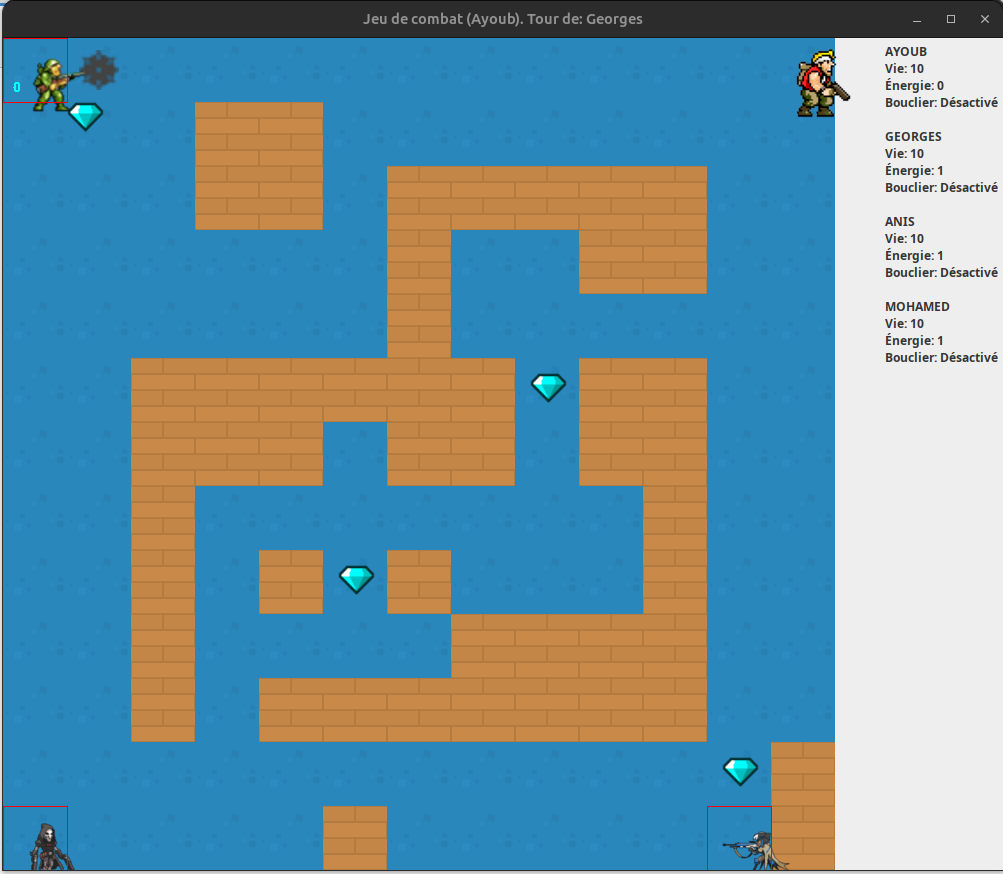
\includegraphics[scale=0.22]{images/interface.png}
    \caption{Résultat de la vue (Interface)}
\end{minipage}
\hfill
\begin{minipage}{0.45\textwidth}
    \centering
    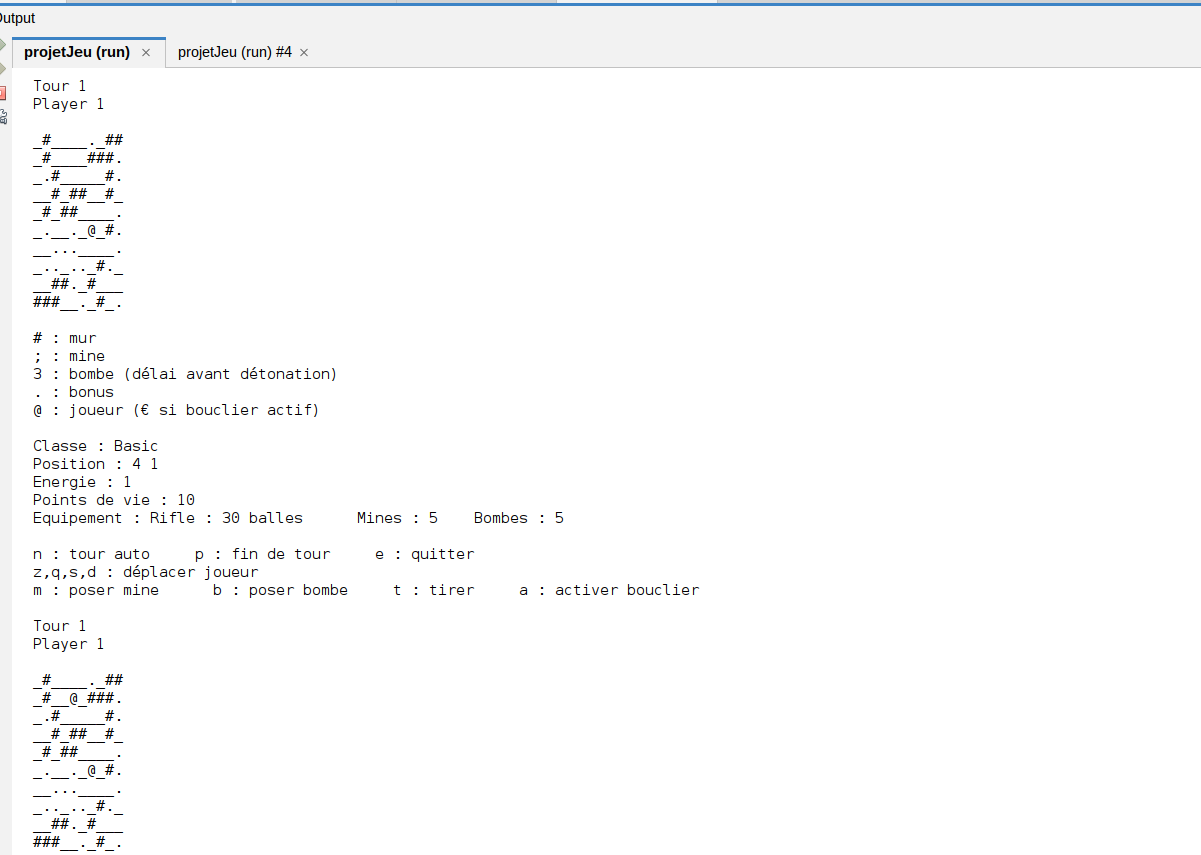
\includegraphics[scale=0.22]{images/terminal.png}
    \caption{Résultat de la vue (Console)}
\end{minipage}
\end{figure}

\begin{figure}[!h]
\centering
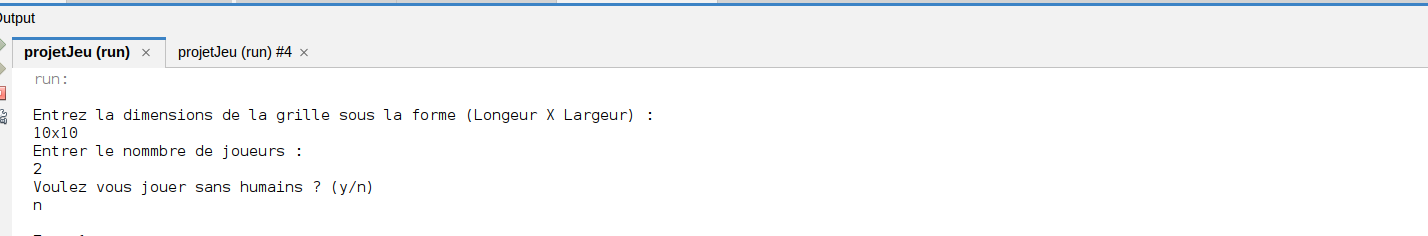
\includegraphics[scale=0.25]{images/choix.png}
\caption{Le choix dans la console}
\end{figure}

\section{Algorithmes non triviaux}

Plusieurs algorithmes complexes sont utilisés dans le projet pour gérer des aspects critiques du jeu. Voici une présentation des principaux :

\begin{itemize}
    \item \textbf{Génération procédurale de la grille} :  
    Implémentée dans la classe \texttt{RandomGridGeneretor}, cet algorithme génère des grilles de jeu en plaçant des éléments (murs, bonus, obstacles) de manière aléatoire tout en respectant des contraintes comme l'accessibilité des chemins entre les points clés.

    \item \textbf{Gestion des grilles partielles avec le Pattern Proxy} :  
    La classe \texttt{GridProxy} limite dynamiquement la visibilité des informations de la grille en fonction du joueur. Chaque joueur voit uniquement les parties découvertes ou accessibles de la grille, nécessitant une gestion fine des permissions.

    \item \textbf{Chargement dynamique des niveaux} :  
    La classe \texttt{LevelHandlerParser} analyse les fichiers XML pour charger les niveaux du jeu. Elle transforme les données structurées en objets manipulables dans le jeu, en s'assurant que les configurations sont cohérentes et sans erreurs.

    \item \textbf{Comportement des joueurs contrôlés} :  
    À travers l'interface \texttt{RandomStrategy}, le comportement des bots est défini, incluant des décisions contextuelles comme le mouvement, l'attaque, ou la défense. Cet algorithme garantit un robot compétitif et adaptable.

    \item \textbf{Gestion des événements avec des listeners} :  
    Les classes \texttt{ListenableModel} et \texttt{ModelListener} implémentent un système d'écoute pour synchroniser la vue avec le modèle. Cela permet une mise à jour dynamique de l'interface utilisateur en réponse aux actions des joueurs.
\end{itemize}

Ces algorithmes illustrent des solutions avancées pour répondre aux défis de la conception et du développement d'un jeu interactif.


\section{Compilation et Exécution}

\subsection{Compilation}
Pour compiler le projet en ligne de commande :\\
Placez-vous dans la racine du projet et tapez les commandes suivantes :
\begin{lstlisting}[language=Bash, frame=single]
ant compile # compilation
ant run     # execution
\end{lstlisting}

\subsection*{Exécution}
Pour exécuter le projet depuis la ligne de commande, accédez au dossier \texttt{dist} et tapez les commandes suivantes :

\subsubsection{Partie Console}
\begin{lstlisting}[language=Bash, frame=single]
java -jar "projetJeuConsole.jar"
\end{lstlisting}

\subsubsection{Partie Graphique}
\begin{lstlisting}[language=Bash, frame=single]
java -jar "projetJeuGraphic.jar"
\end{lstlisting}



\end{document}